\documentclass[UTF8]{ctexart}

\usepackage{CJK}
\usepackage{ctex}

\usepackage{geometry}% 版面大小
\geometry{a4paper,scale=0.7}

\usepackage{graphicx}
\graphicspath{{assets/}}
\usepackage{caption2}
\usepackage{subfigure}
\usepackage{float}

\usepackage[hidelinks]{hyperref}

\usepackage{listings} % packages for code blockings
\usepackage{xcolor}

\title{\textbf{作业2-1}}
\author{刘时宜 201180078}
\date{\today}

\begin{document}
    \maketitle
    \tableofcontents
    \section{验证镜像源速度}
    通过ping命令,验证三个镜像源的速度。
    \begin{figure}[H]
        \centering
        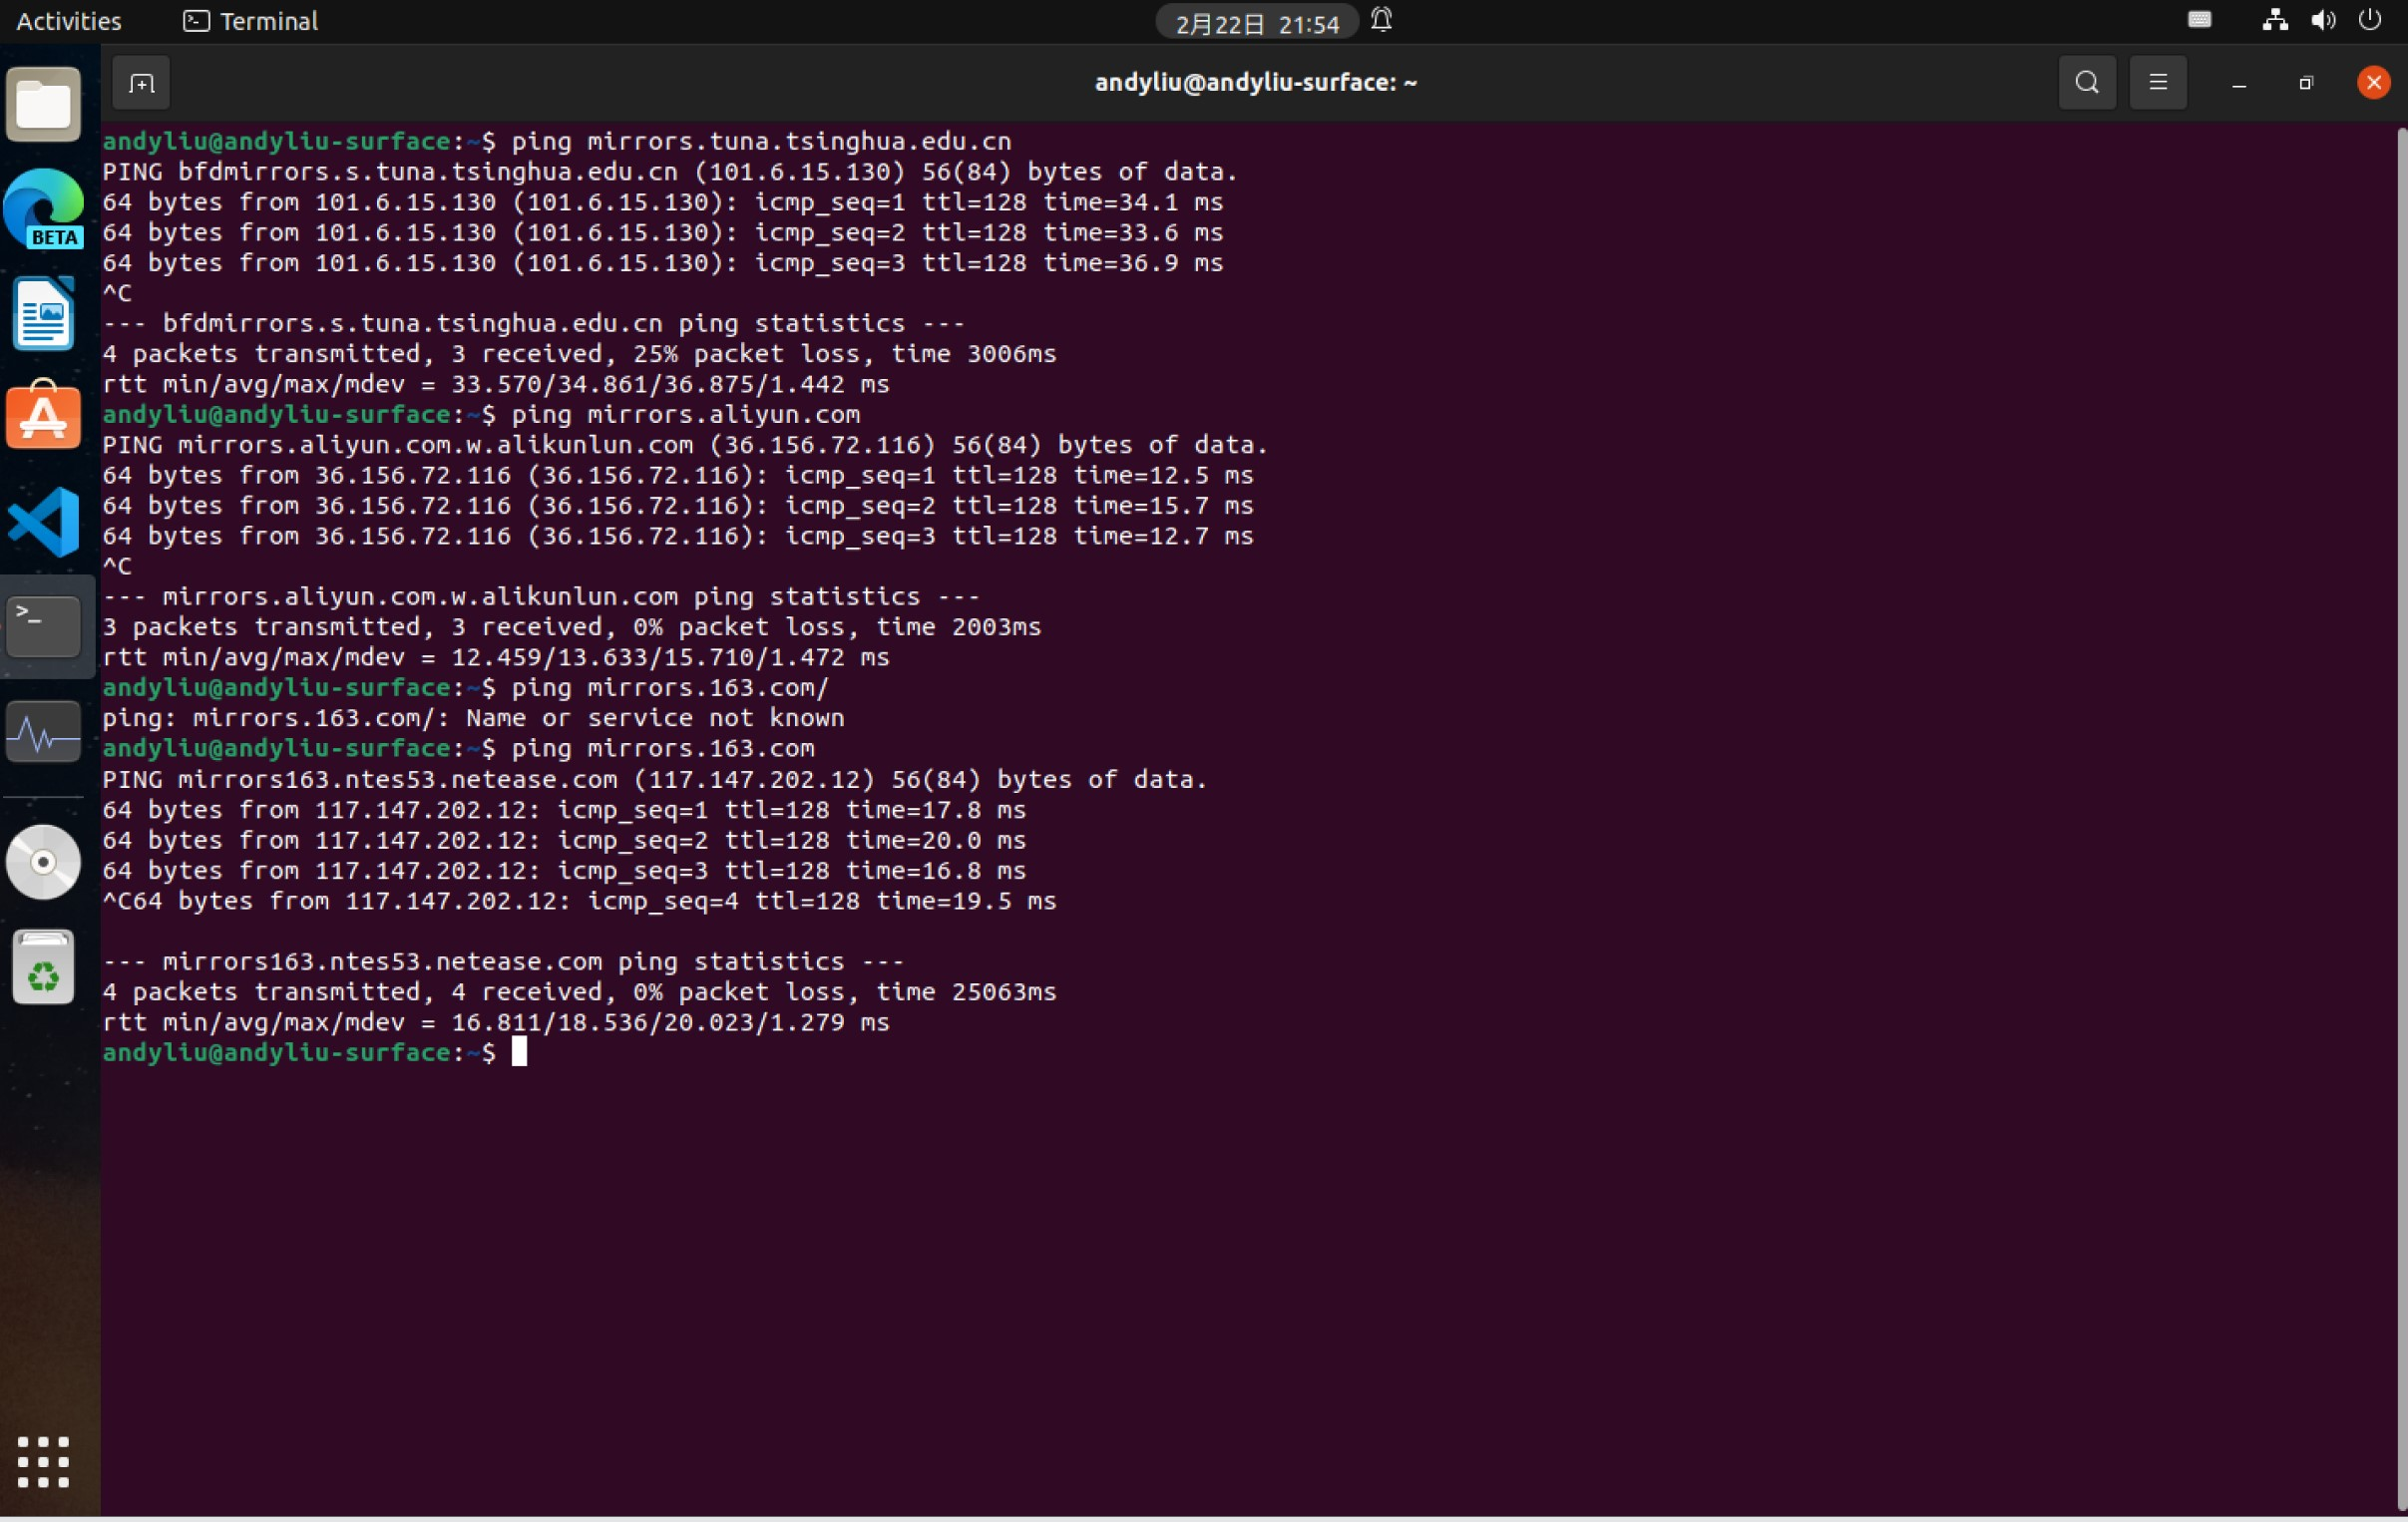
\includegraphics[width=0.8\textwidth]{ping.jpg}
    \end{figure}
    从ping执行结果可以看出,阿里云的往返时间(RTT)均小于16毫秒,为几个镜像源中最快的。
    

    \section{更换镜像源}
    但是由于阿里云没有给出个人使用的ubuntu版本的换源方法,故使用清华镜像源进行换源。参照清华镜像源中给出的换源方法如图\ref{thu mirror}所示。
    \begin{figure}[H]
        \centering
        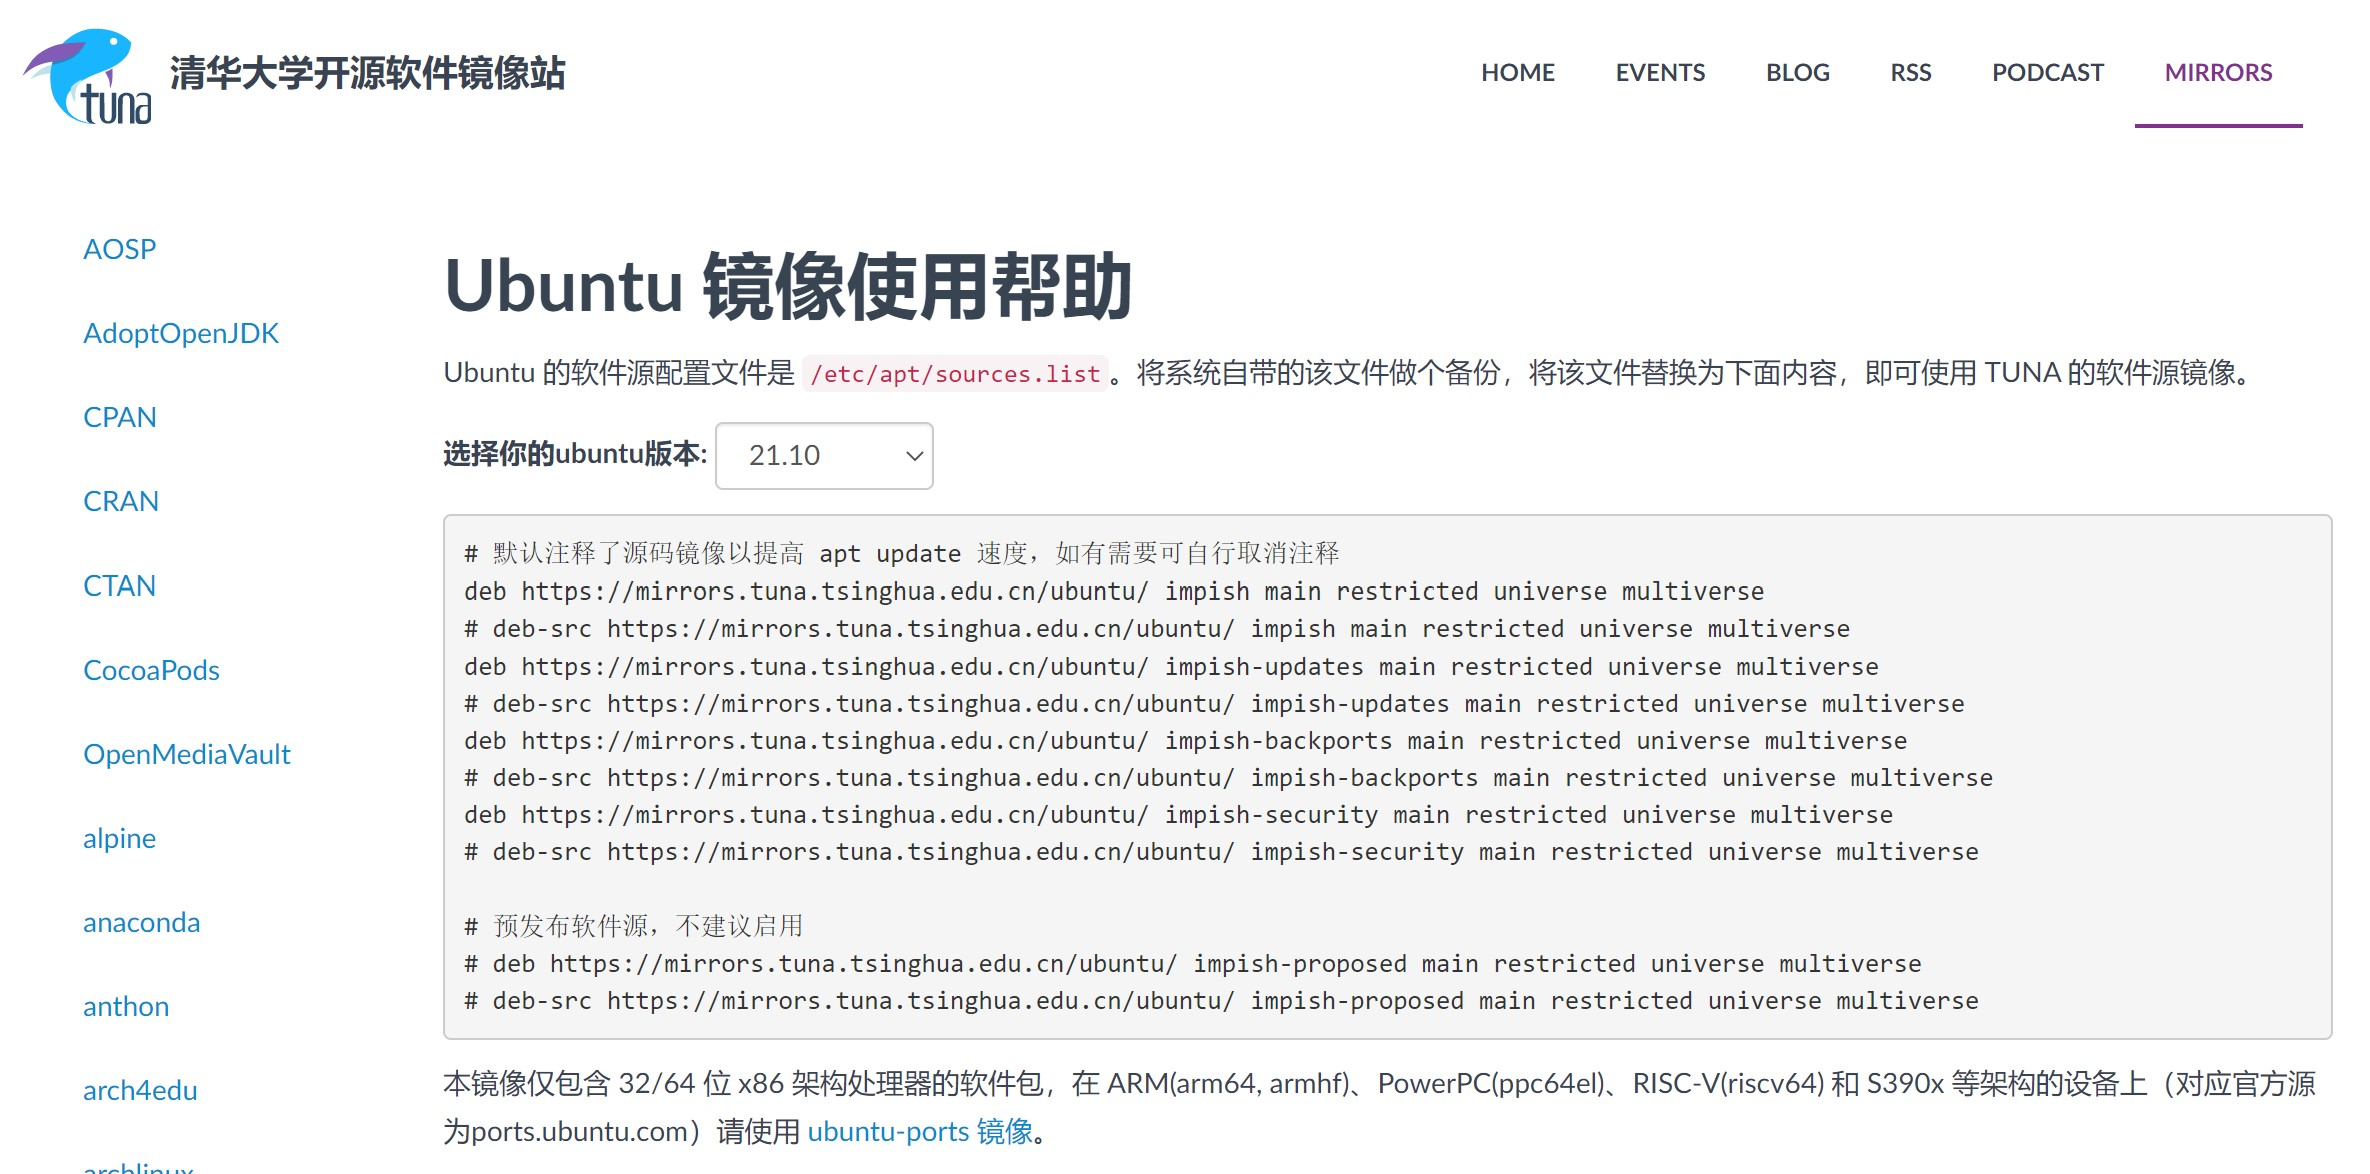
\includegraphics[width=0.8\textwidth]{thu mirror.jpg}
        \caption{清华TUNA镜像源中给出的换源说明}
        \label{thu mirror}
    \end{figure}

    使用vim命令调用vim编辑器修改/etc/apt/sources.list文件中的内容,修改后保存,使用cat命令确认保存成功,如图\ref{source list}所示。
    \begin{figure}[H]
        \centering
        \subfigure[vim编辑器]{
        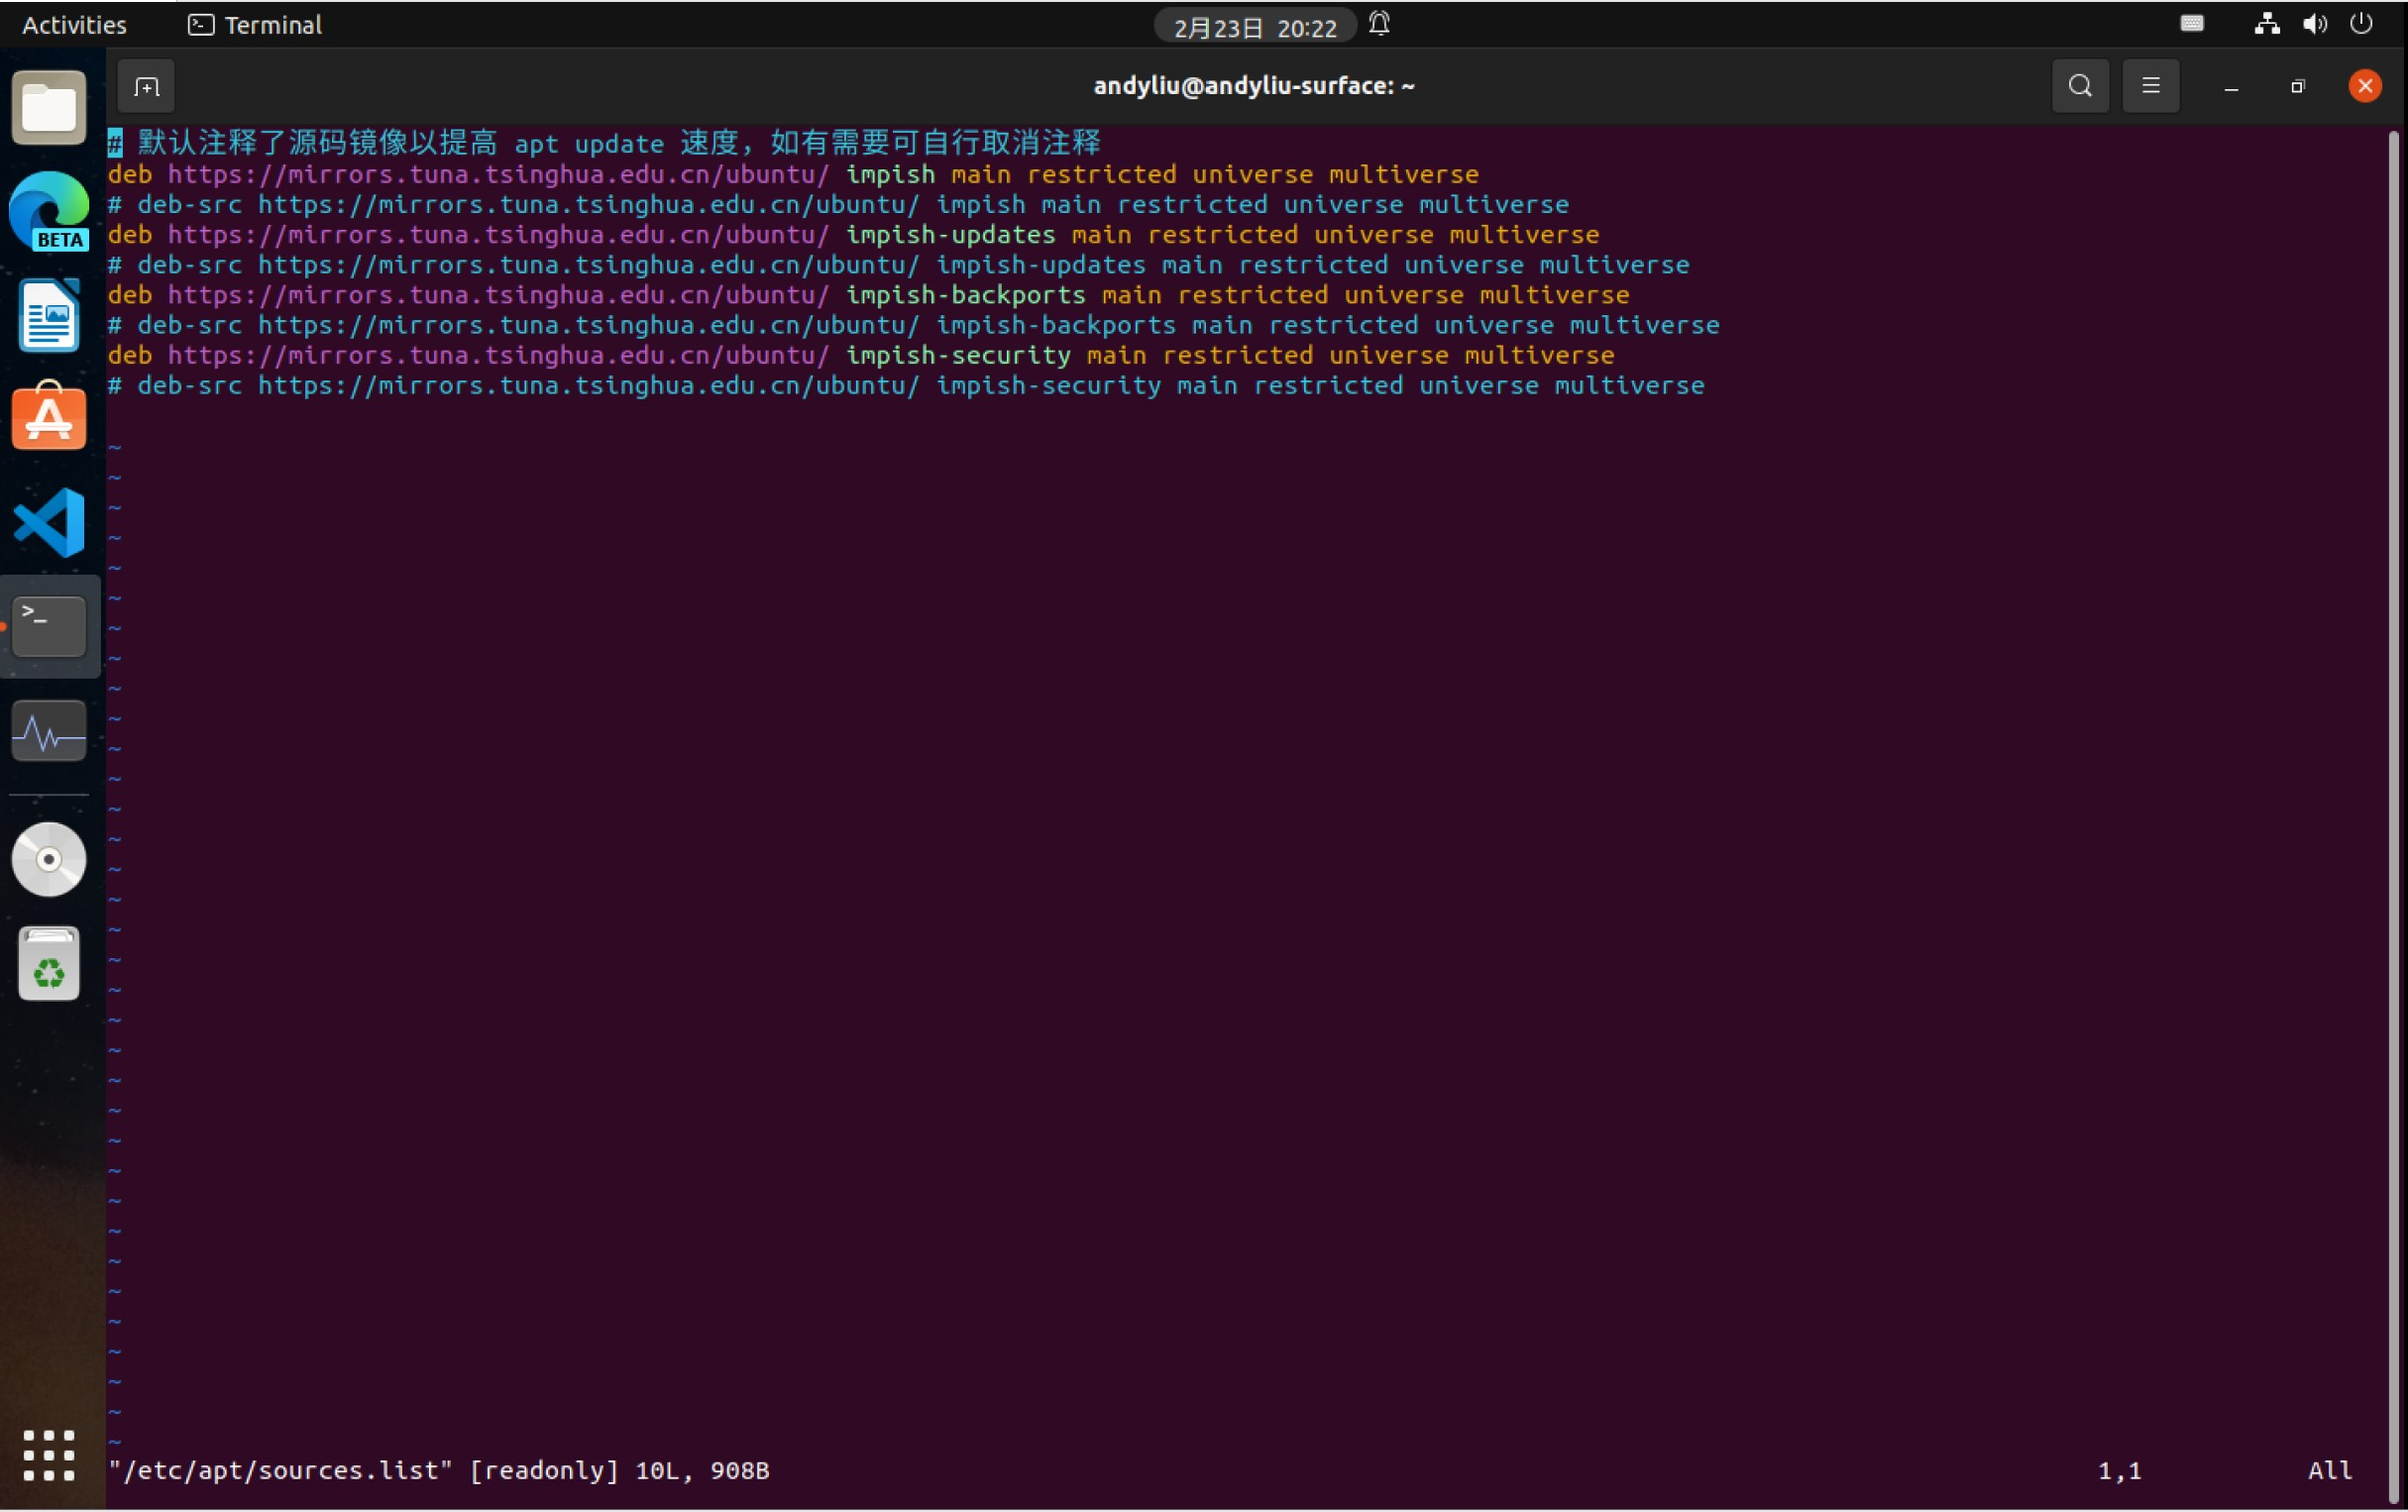
\includegraphics[width=0.45\textwidth]{sourcelist.jpg}}
        \subfigure[bash命令]{
        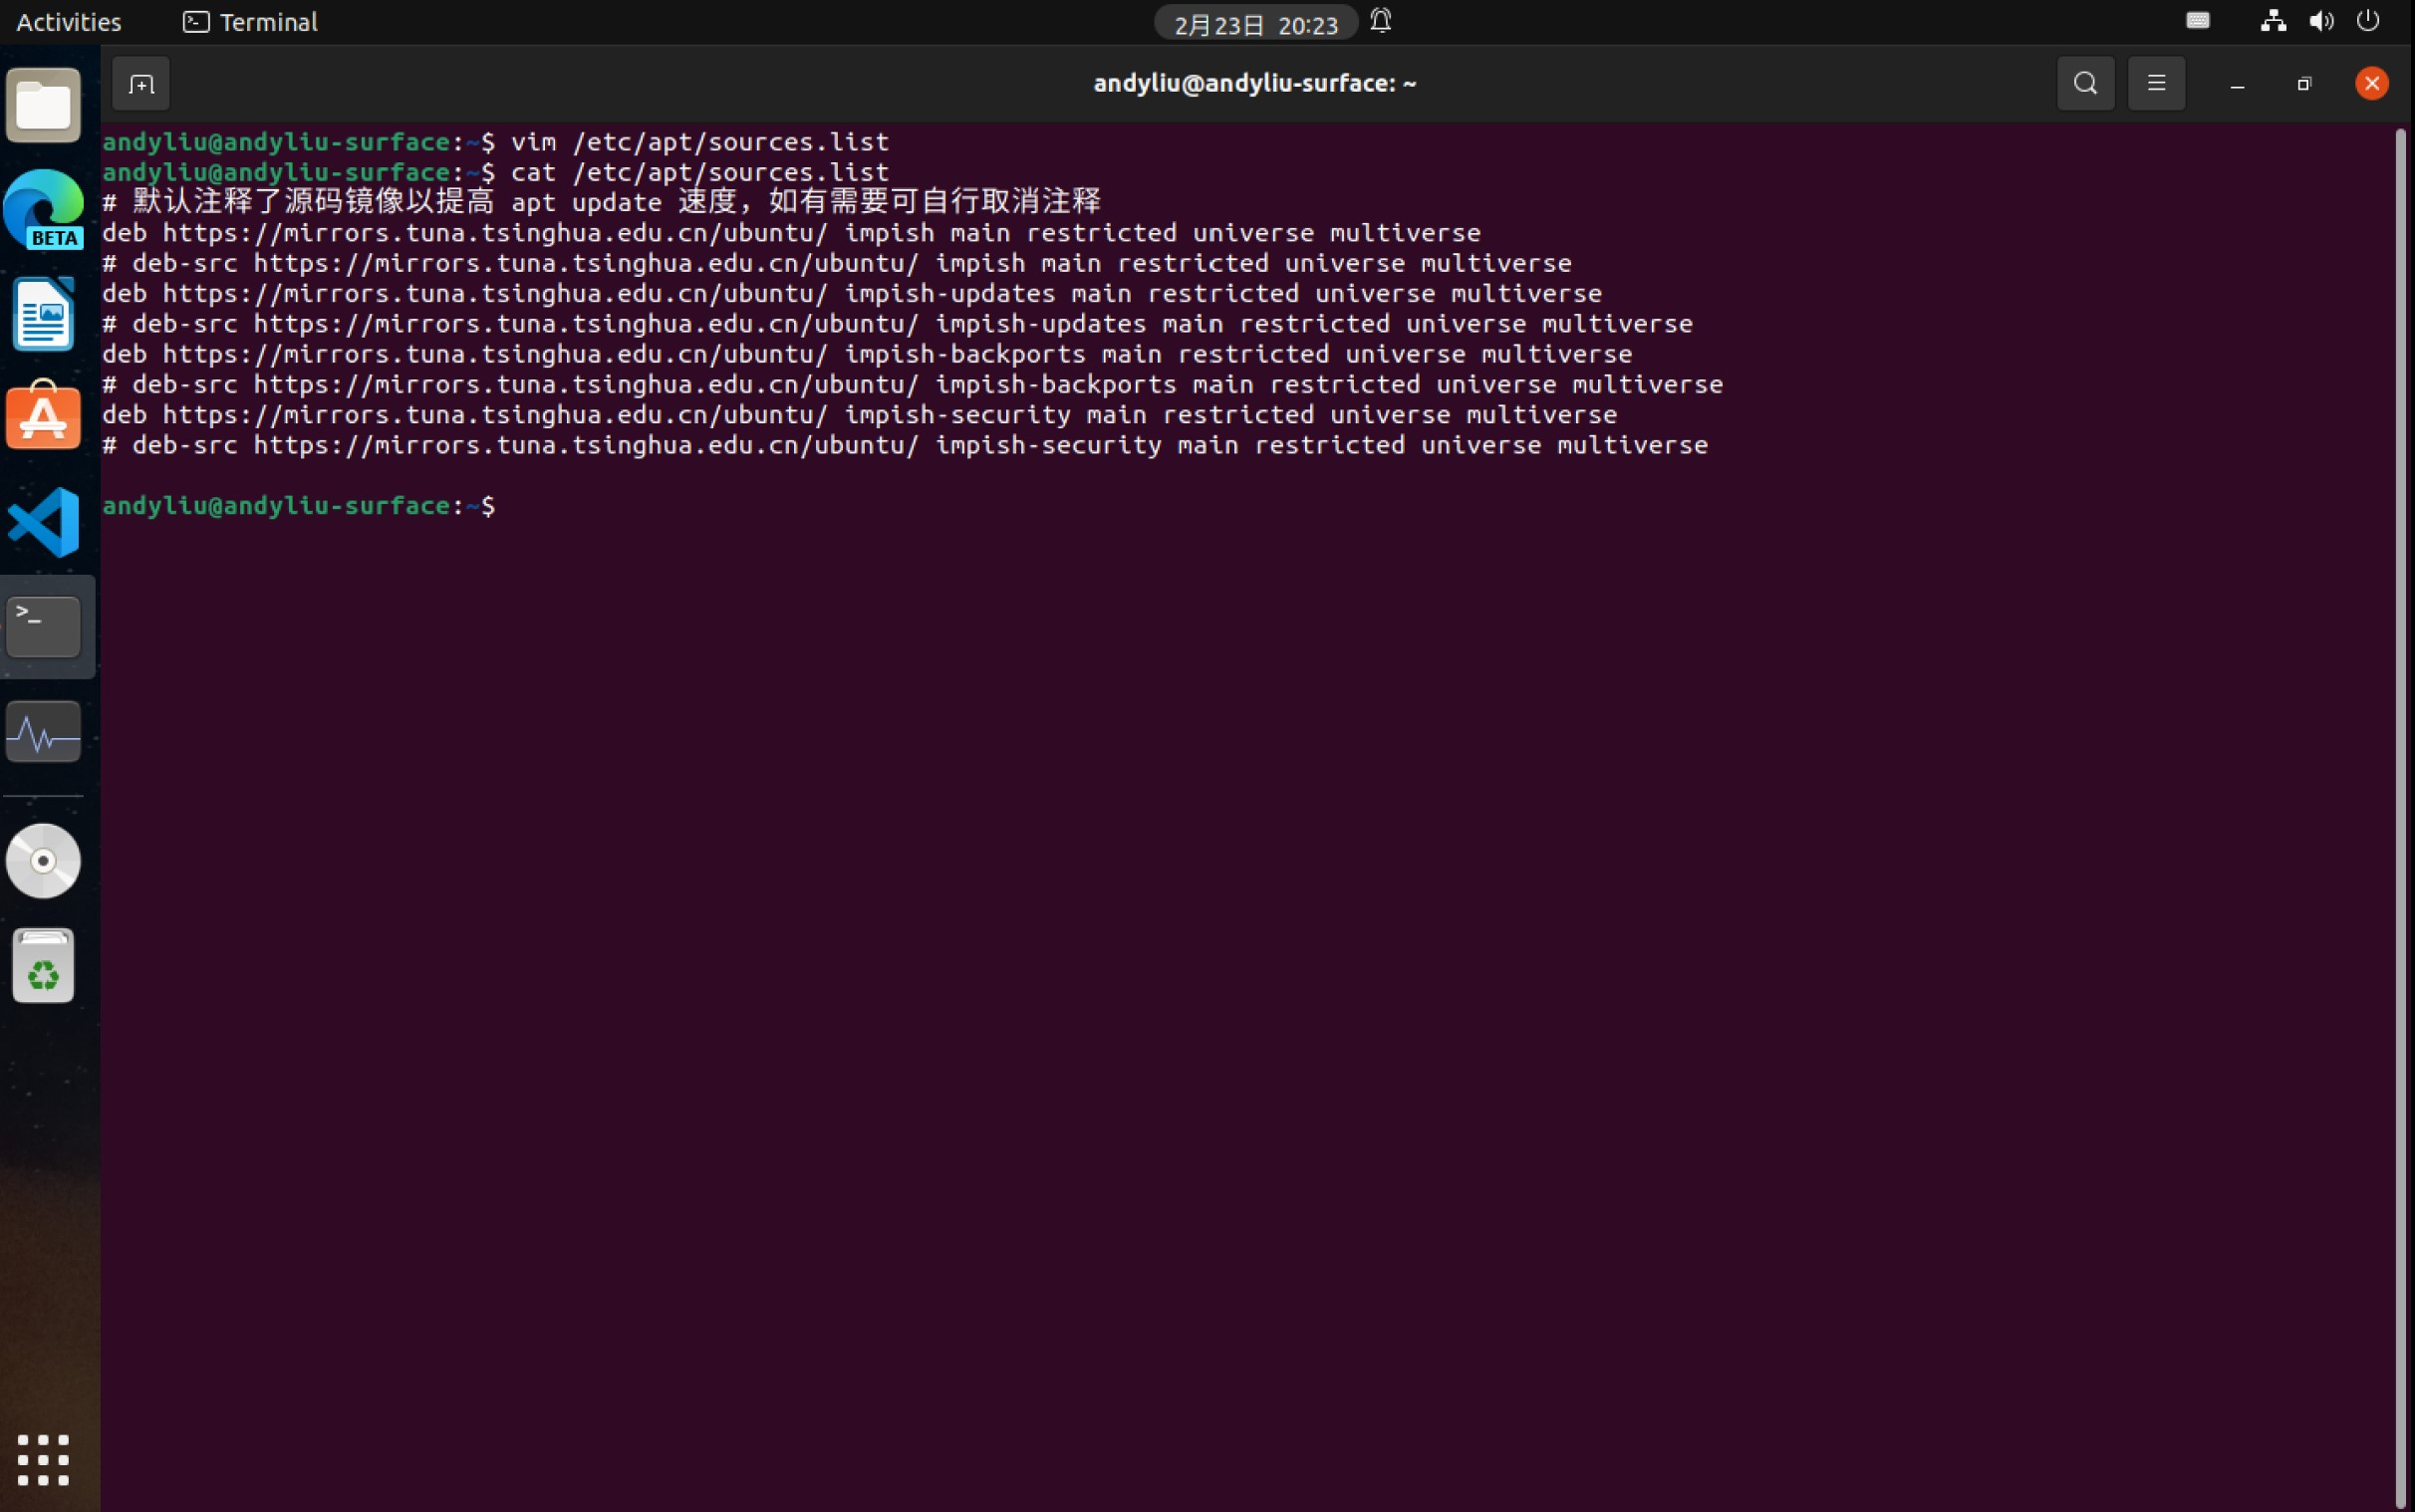
\includegraphics[width=0.45\textwidth]{bash.jpg}}
        \caption{修改apt库源}
        \label{source list}
    \end{figure}

    更新包索引并安装相关程序,如图\ref{update install}所示。
    \begin{figure}[H]
        \centering
        \subfigure[更新索引]{
        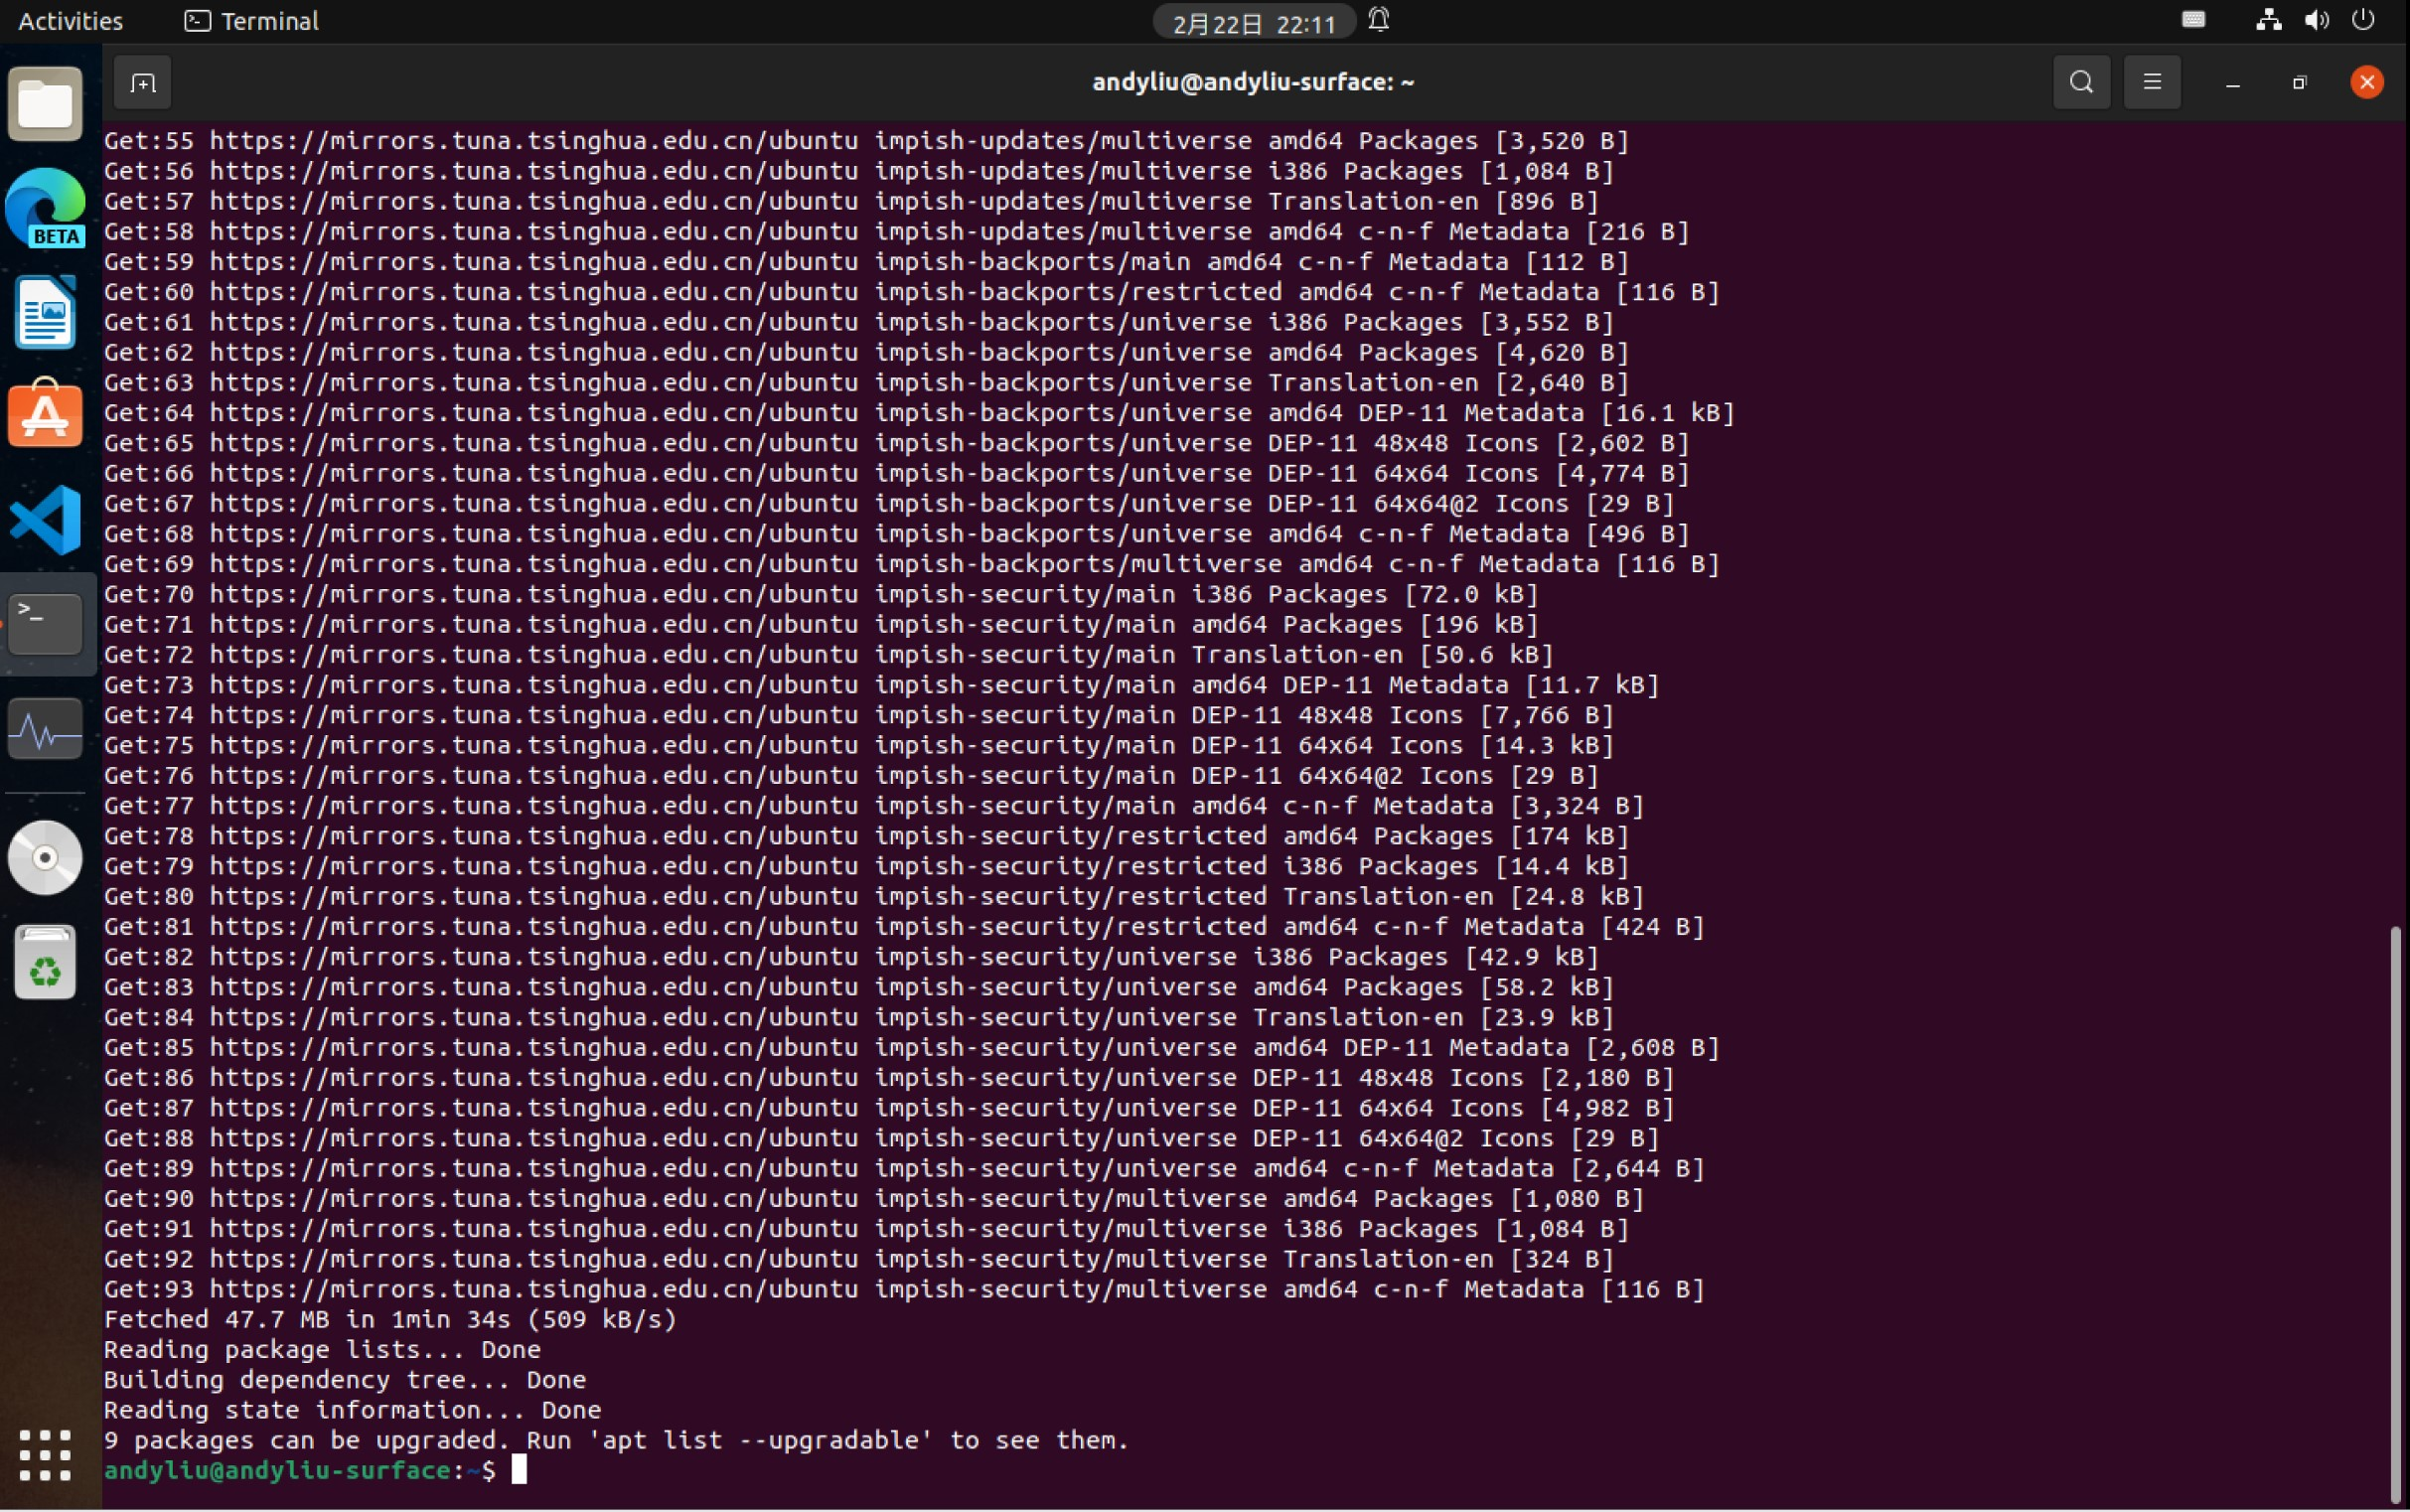
\includegraphics[width=0.45\textwidth]{apt upgrade.jpg}}
        \subfigure[安装程序]{
        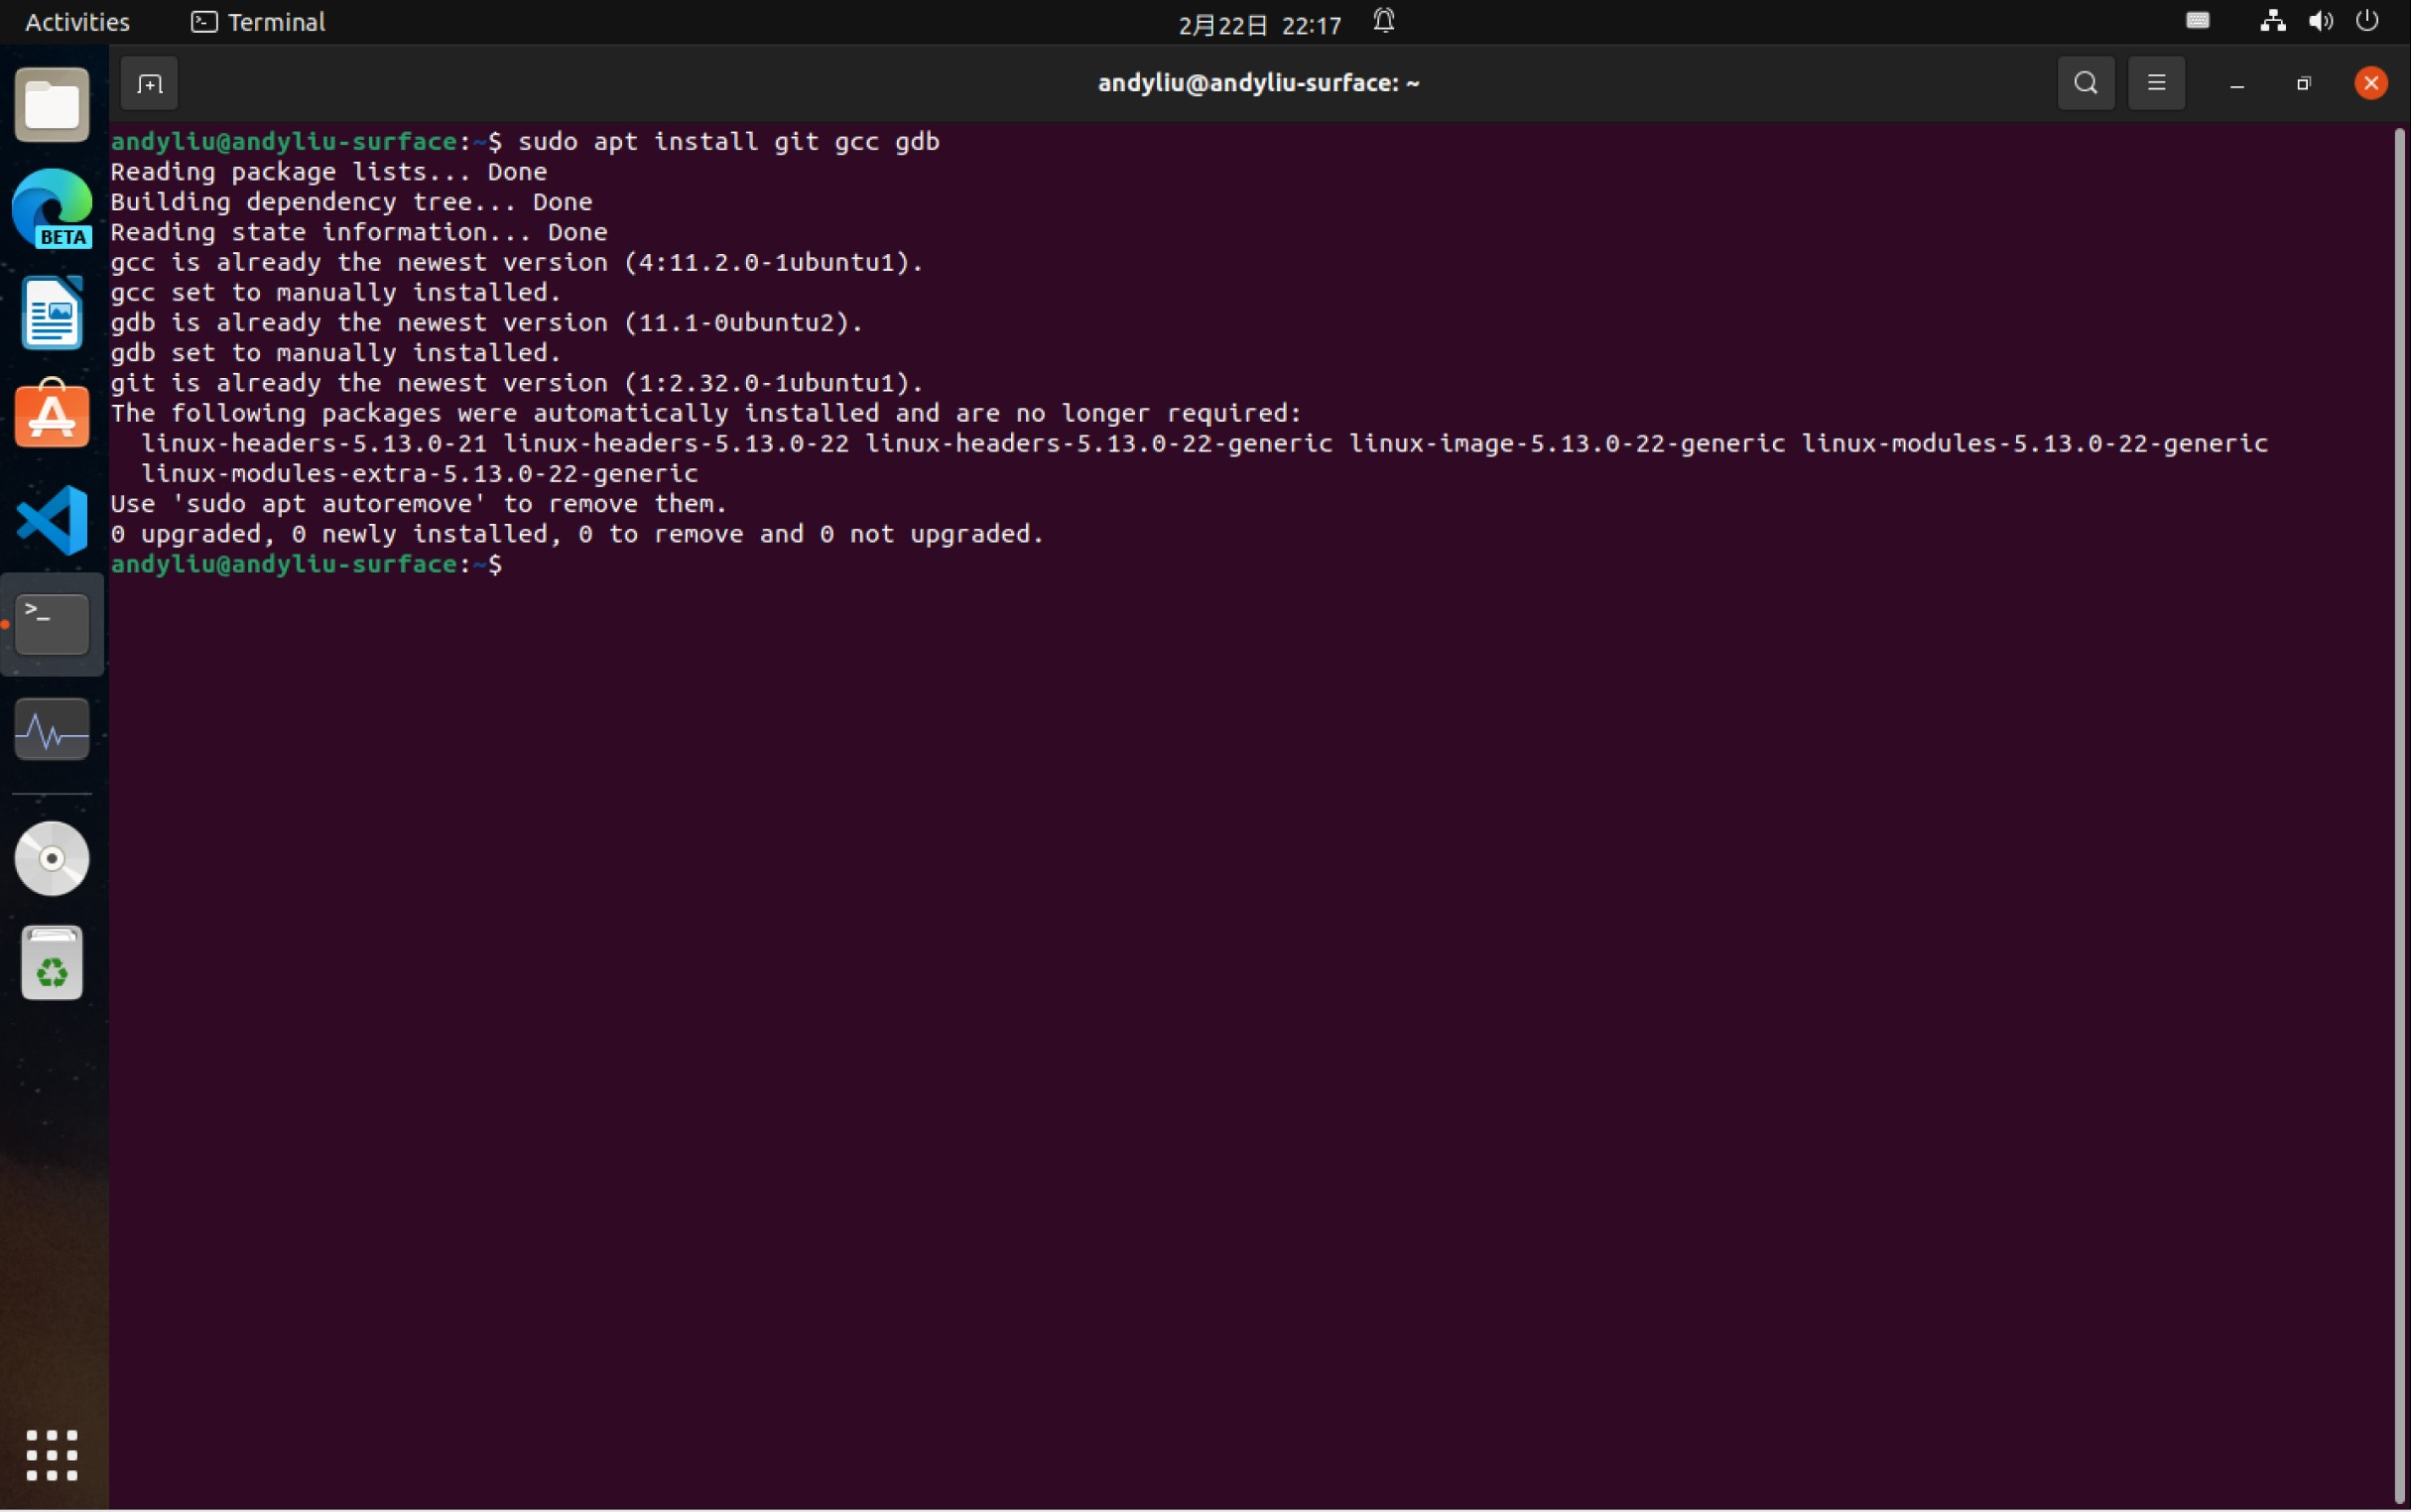
\includegraphics[width=0.45\textwidth]{apt install.jpg}}
        \caption{更新索引、安装程序}
        \label{update install}
    \end{figure}

    \section{编写程序并运行}
    使用touch命令新建文件、vim编辑器编辑c源文件,使用cat确认保存成功,使用gcc编译c代码,然后运行程序。相应命令行操作过程以及vim编辑器编辑界面如图\ref{programming}所示。
    \begin{figure}[H]
        \centering
        \subfigure[bash]{
        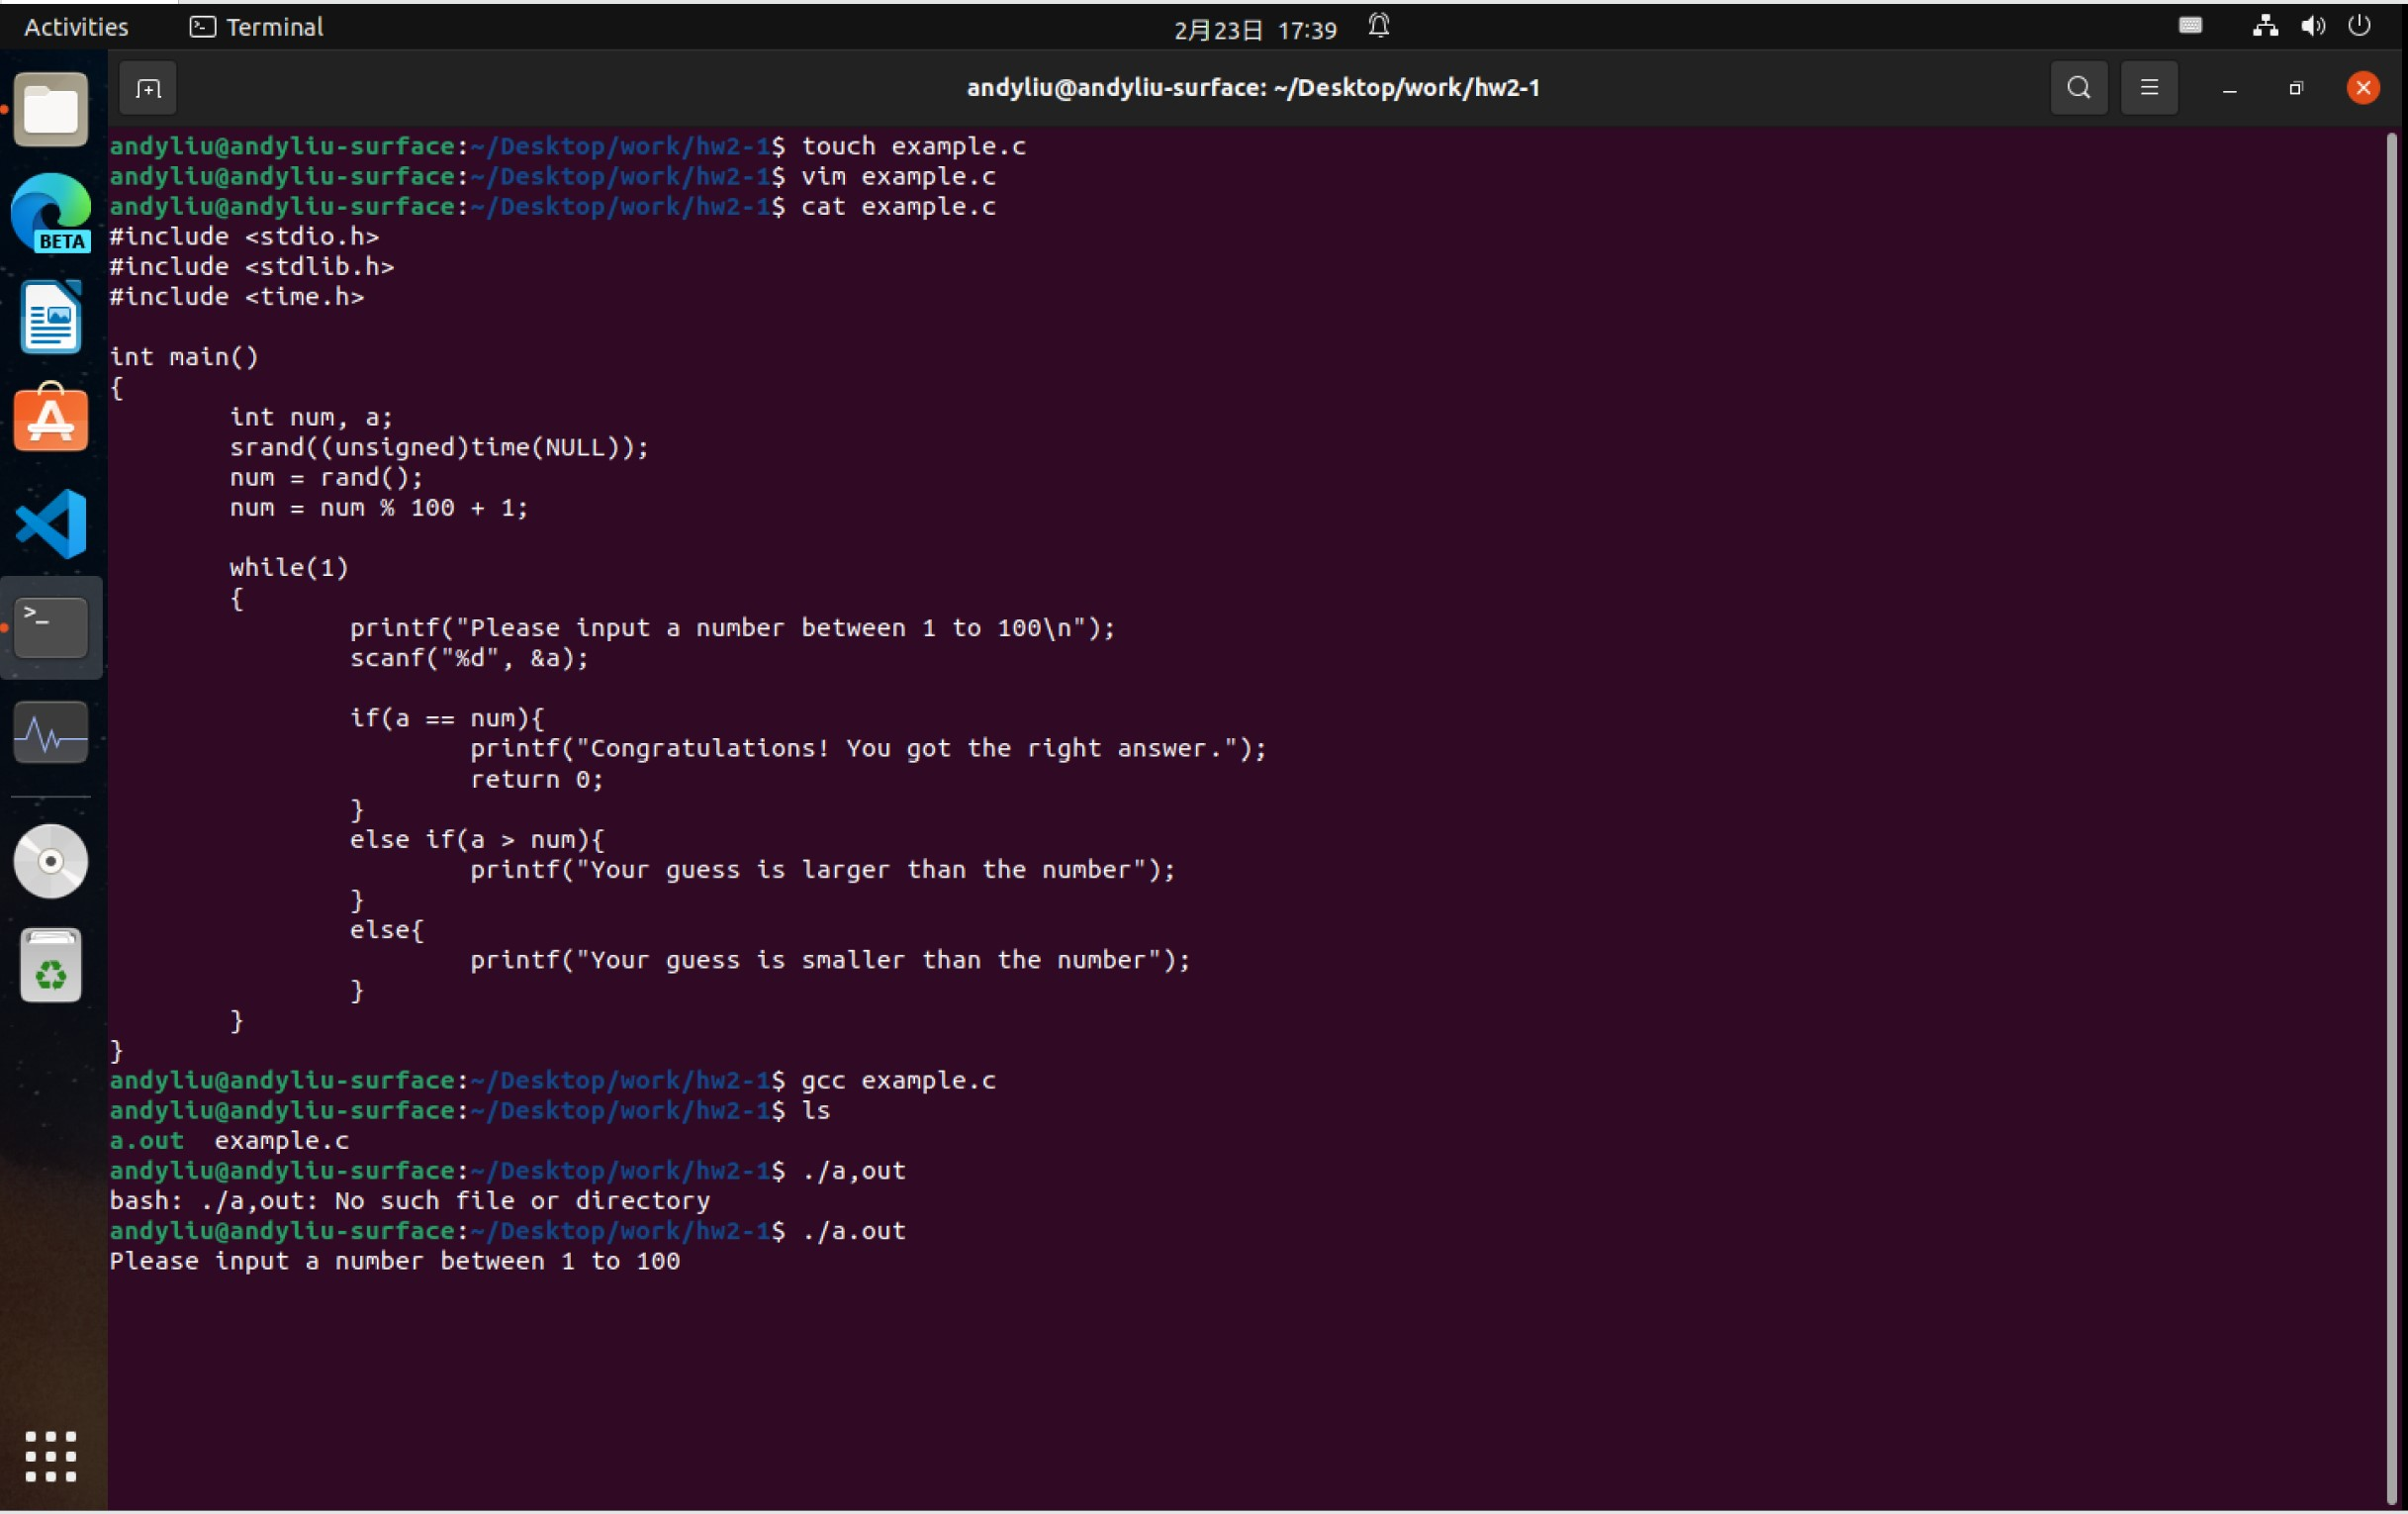
\includegraphics[width=0.45\textwidth]{instructions.jpg}}
        \subfigure[vim]{
        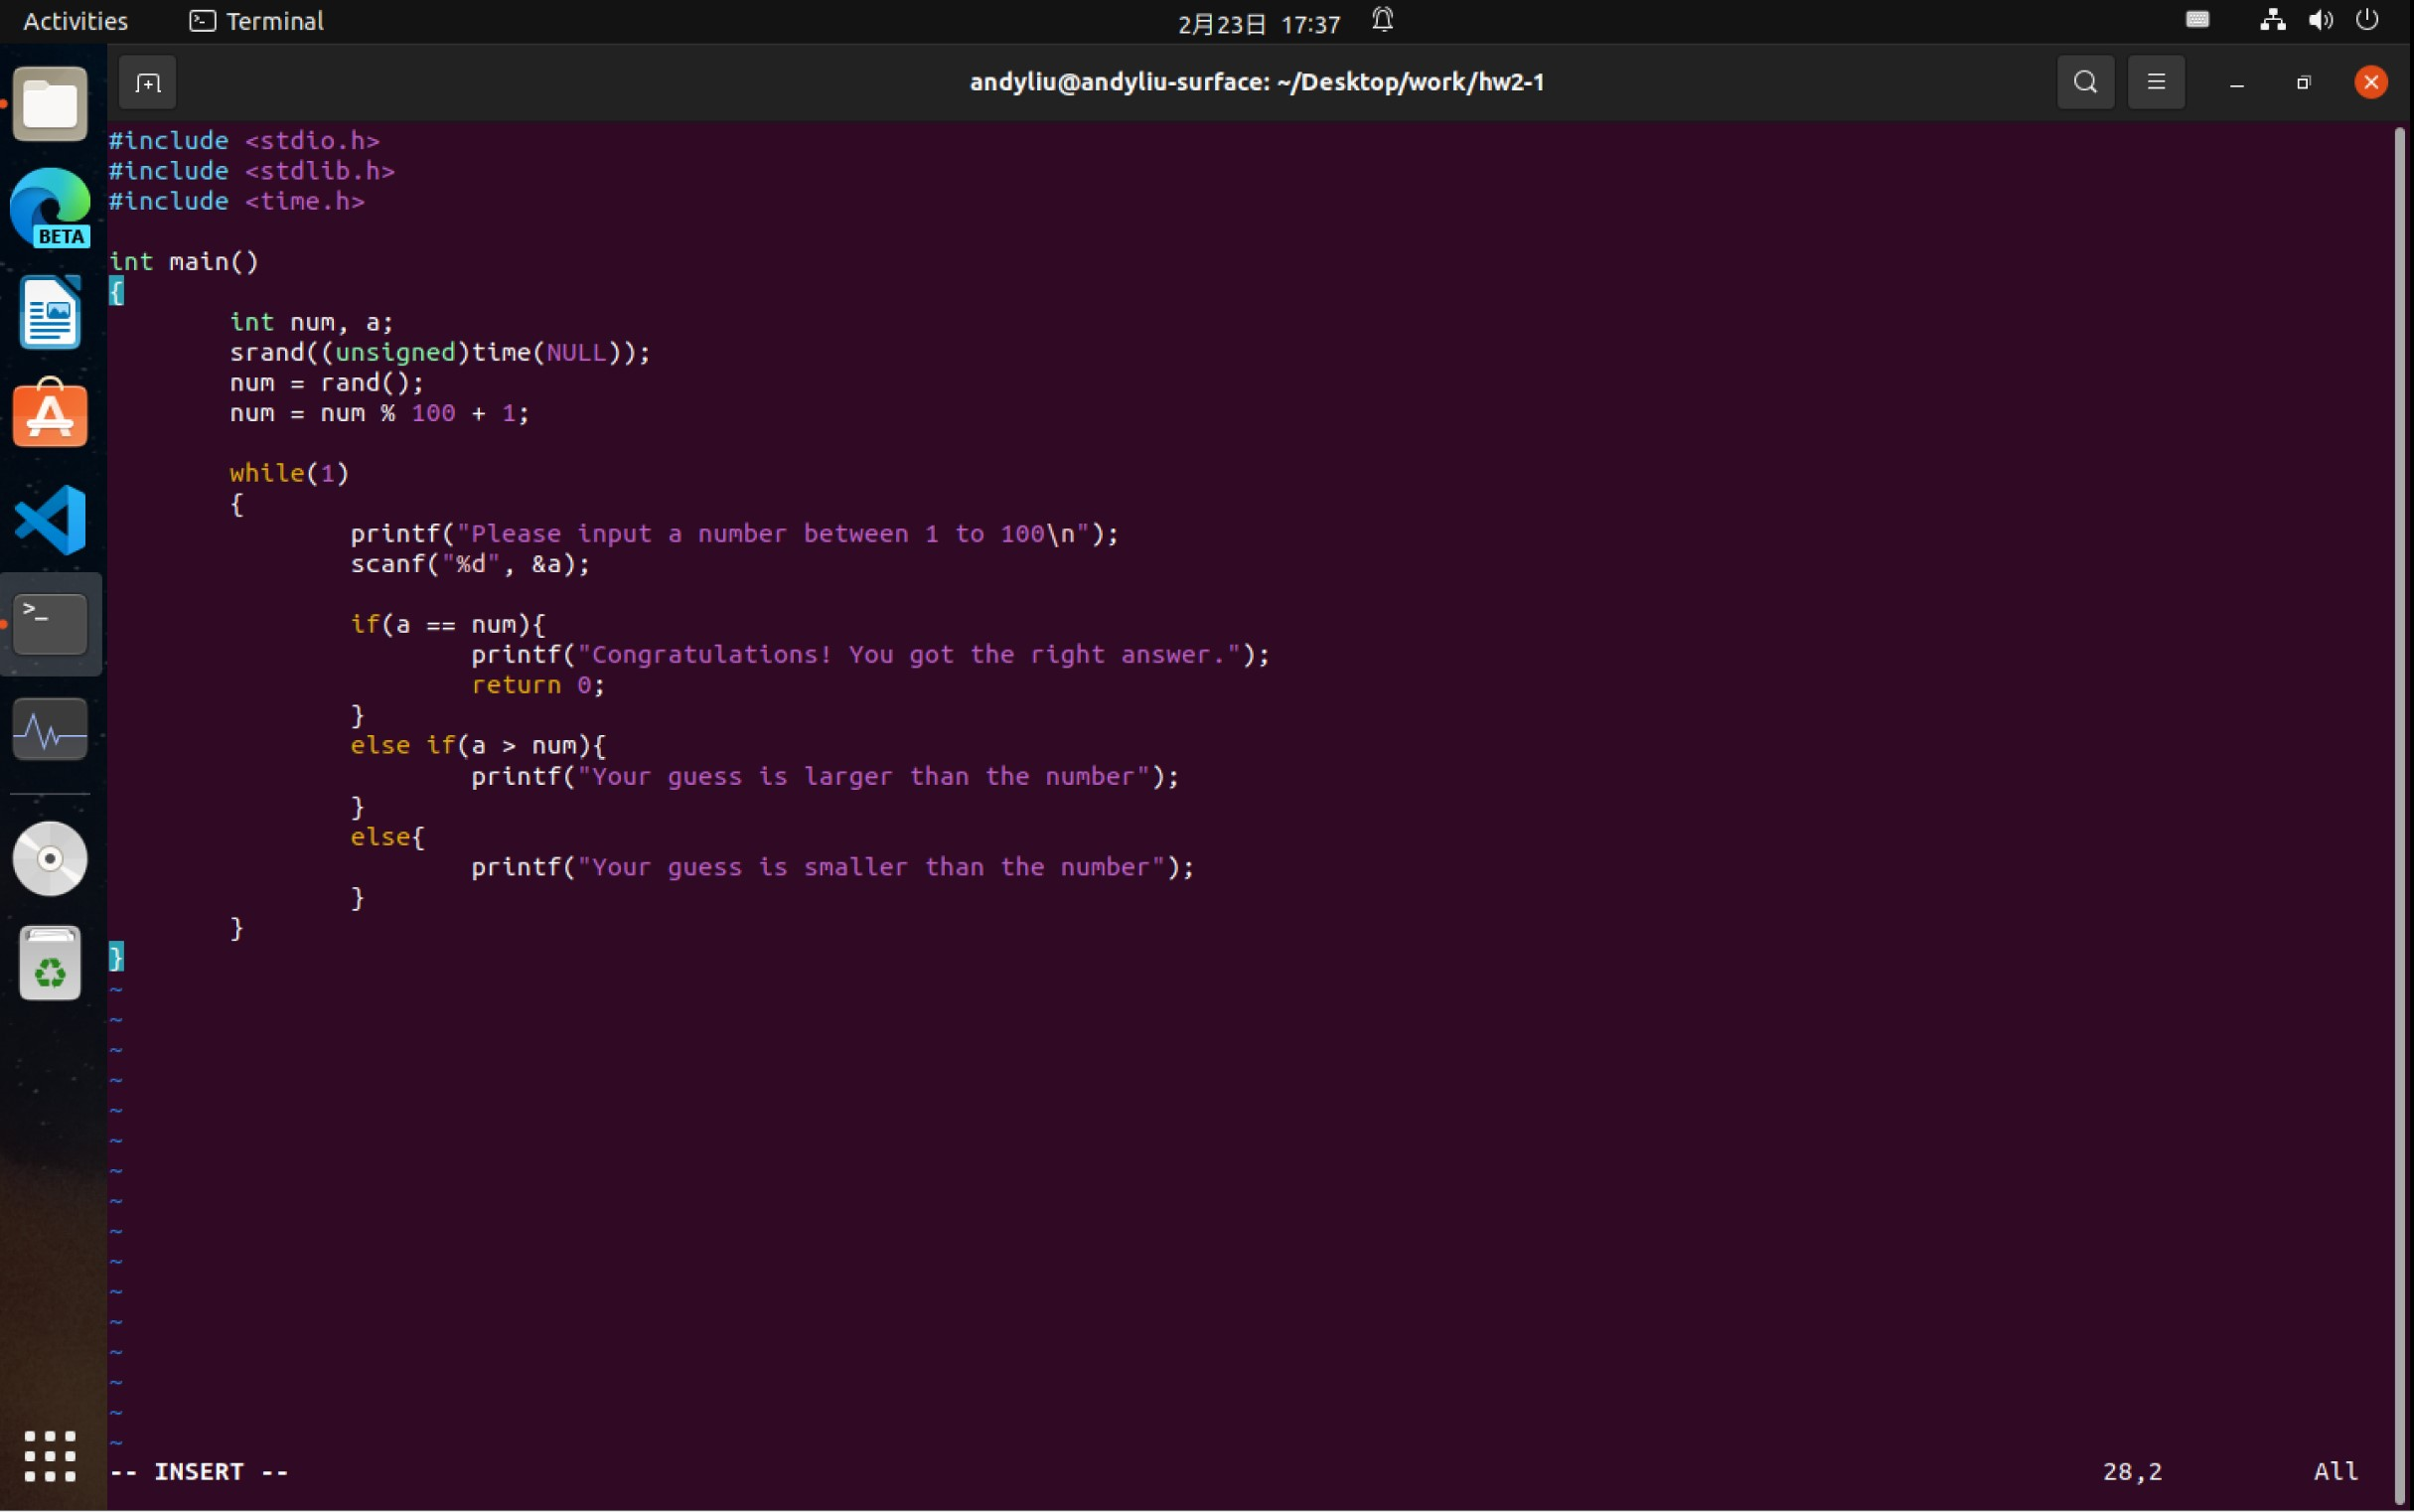
\includegraphics[width=0.45\textwidth]{program.jpg}}
        \caption{编写、编译并运行程序}
        \label{programming}
    \end{figure}

    期间,用到vim的命令及操作方法有:
    \begin{enumerate}
        \item 进入vim界面后,按i进入insert模式编辑源代码
        \item 按住ctrl键以及上下左右键以词为单位快速移动光标
        \item 在命令模式下,输入dd删除整行
        \item 编辑完成后,使用:wq命令进行保存后退出的动作。
    \end{enumerate}

    一次完成的程序运行过程如下图所示:
    \begin{figure}[H]
        \centering
        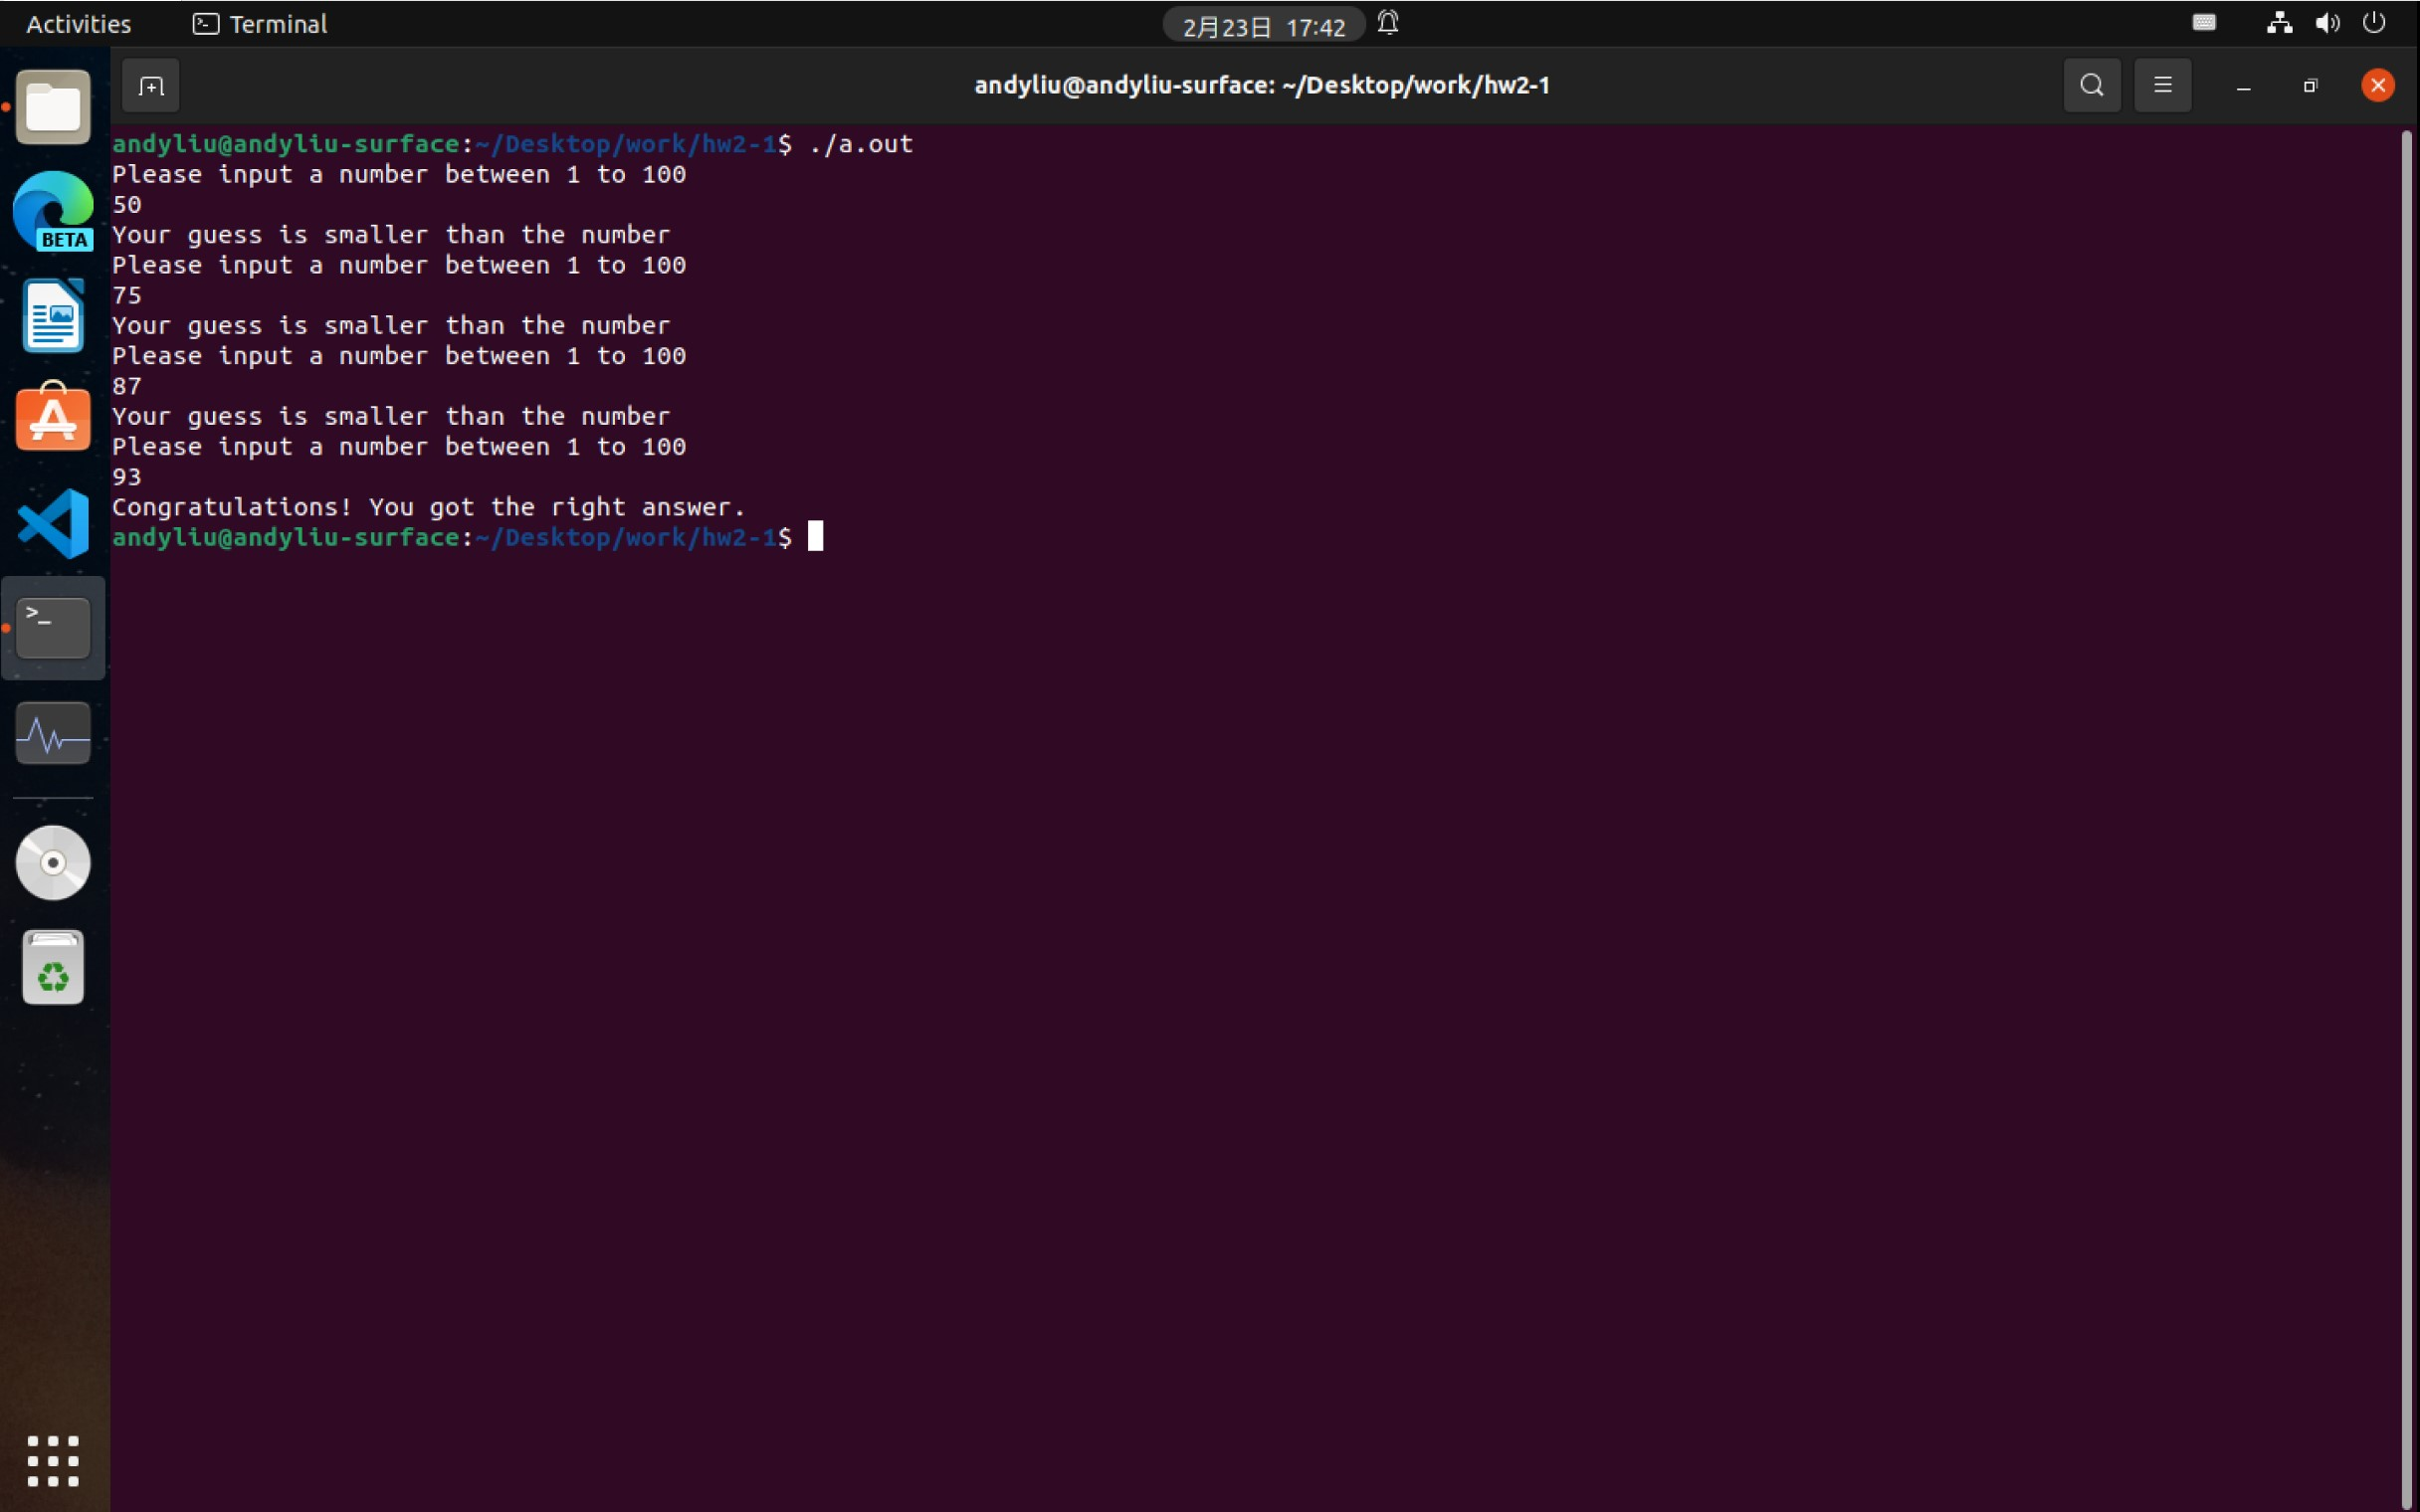
\includegraphics[width=0.8\textwidth]{running.jpg}
    \end{figure}


\end{document}